\section{Introduction}

Our societies are fueled by energy. Historically, fossil fuels offered a relatively easy to access, store and use energy for decades, bringing a solution to this energy issue.

The rising awareness of the climate change, mostly caused by the release of large amounts of greenhouse gases conducts to a paradigm shift. To meet climatic goals, strict limits on emissions have been established, consequently limiting the prevously endless source of energy that were fossil fuels over the long term \cite{ar6-ipcc-wg3}. This directly impacts the solutions depending on their combustion, releasing massive amounts of carbon dioxide.

The solutions to compensate for the lacking energy generation, that from now on should not derive from fossil fuels, are renewable energy sources. These refer to every energy generation technique originating from a renewable source, such as the sun, the wind and the rivers. However, the production of these units is not systematically sustainable. For example, the photovoltaic cells necessary for the exploitation of the incoming solar energy are pretty difficult to recycle, making them rely on specific materials that are not obtainable renewably. Still, their use on a complete lifetime, and increasing capabilities in recycling, justifies the investment in their construction.

In this context, a meaningful increase in the electricity produced from such energy sources is to be expected, particularly from the most prominent ones:
\begin{itemize}
    \item the sun, through photovoltaic panels,
    \item the wind, through on-shore and off-shore wind turbines,
    \item rivers, through hydroelectric dams,
    \item biomass, through adequate units, and
    \item geothermal energy, through geothermal power stations.
\end{itemize}

The third one, due to its dependency on the geographic context, will however not expand foerever, as there are not illimited spots to build such dams. In this work, the biomass and geothermal energy sources, less common for the time being, are not considered.

One thus falls back to photovoltaic and wind energy, but both have a major, trivial drawback: they rely on the sun and the wind, respectively. And this is a significant concern, because the amount of energy that can be generated by exploiting these is variable, hence their designation as variable renewable energy sources, or VRES.

That variability does not necessarily involve poor predictability, for example, there is on average more photovoltaic production potential during summer. On a daily scale as well, with the day night cycle. Weather forecasts can be taken advantage of in order to predict wind turbines' production.

% The larger variability of the power output of VRES constitutes an issue, because modern electrical system is dictated by consumers' demand. And to do so, electricity generators are dispatched in real-time, so that the production always matches the demand on the network. This technique works because the relevant power plants can be started and shut down on demand, almost at any time. With VRES, this assumption drops, as an additional wind turbine cannot be started if there is no wind, nor a photovoltaic panel be turned on during the night.
The idea of residual load, the difference between the actual load and the amount of energy that can be provided from renewable sources. This residual load fluctuates, therefore needing conventional electricity units to be dispatched in real time. But since these units have start-up and shut-down costs, minimizing these remains attractive. Hence, flattening the residual load curve is desired, what governs the dispatch the units available on the network.

\subsection{Flexibility assessment in energy system models}

As explained before, higher shares of VRES in the electricity production mix create the additional challenge, that is the handling of the partlially predictable variability of wind and sun energy. 

This handling requires a larger flexibility of the electrical system, that is, a better ability to adapt to both anticipated and unforeseen changes in the demand and supply \cite{irena}.

Existing mechanisms to improve the flexibility of a power system include:

\begin{itemize}
    \item Use of the regular dispatchable energy production plants to compensate for the energy deficit that may arise from VRES. Plant characteristics play a role to address short term drops in production, as some start up time might be required \cite{flexibility-storage-planning}.
    \item Large interconnected electricity networks, that are able to smooth the VRES power output. There may be not enough sun in some region, creating a deficit, while there is too much in the neighboring country. By connecting them, the overproduction will compensate the unerproduction of the other \cite{flexibility-connection}.
    \item Energy storage facilities. Of course, storing the produced energy for later use is an easy way to account for the intermittency of the production. Typically, storing solar energy during day time to be used in the night. These technologies include pumped hydro-storage, batteries, compressed air. While pumped hydro-storage units are the most common, their very limited expansion options make them unlikely to grow in the future \cite{flexibility-demdandside-forecasts-storage}.
    \item Acting on the demand, in the extent that it can change its shape by promoting policies to the end users. Such policies focus on flattening the daily demand curve, facilitating the energy production dispatch. Typically, asking to delay greedy devices like dishwashers until night, where the overall demand is lower. But this could extend to other domains, such as electric vehicles charge, heating and cooling etc \cite{flexibility-demdandside-forecasts-storage}.
\end{itemize}

The two main consequences of insufficiently flexible energy systems are curtailment, when there is too much energy produced, and load shedding, when there is not enough electricity to satisfy the demand. In case of load shedding, parts of the grid may be entirely shut down.

\subsection{Short-term dispatch models}

There exist tools built in order to assess the behaviour of large electrical systems, that are subject to higher share of VRES. These tools typically aims at predicting the electricity flows, dispatching available power plants in order to match the production to the demand. 

For these purposes, such tools typically set low time steps, e.g. 1 hour, and their simulation period spans up to one year \cite{short-term-dispatch-1}. This level of granularity is required in order to capture sufficiently well the variations in the availability of variable RES. In association, significant levels of details are modelled, like simulating every existing units. 

Their scope might range from the electrical system only, to the entire energy system, hence encompassing for example heating, transportation, and industry matters. Some also include economical considerations \cite{Antares}.

And from there on, some higher level metrics can be computed, and in particular, we are interested by:
\begin{itemize}
    \item the curtailment, that is, the energy produced in excess while the electricty demand was already met, that end up wasted, and
    \item the lost load, that is, the energy that could not be produced, hence some demand could not be served.
\end{itemize}

The Antares simulator, PLEXOS and MAON models are examples of such tools. Among them, the Dispa-SET model \cite{dispaset} is selected for this work. Dispa-SET is open-source, and focused on balancing problem in the European grid specifically.

This model is formulated in linear programming, that is, a set of linear constraints are defined and an objective function is given. The solver inputs both of these and computes the parameters values that maximize the objective function while matching the constraints.

\subsection{Integrated assessment models}

On another level, integrated assessment models (IAM) aim at estimating the evolution of large, intricated systems involving a lot of different interconnected areas and actors. These are often multidisciplinary and require a lot of modelling choices.

In particular, some IAM attempt to model the evolution of the whole society, from a socio-economical perspective, including environmental aspects and energy concerns. MESSAGEix, GCAM and MAgPIE are examples of such models that have been used in the IPCC reports \cite{GCAM} \cite{MESSAGEix} \cite{Antares} \cite{ipcc-thing}.

Within this category of IAMs, the MEDEAS model \cite{MEDEAS} is selected for this work, being open-source as well and providing a specific european model.

MEDEAS is expressed in terms of systems dynamics, that is, the evolution of the state of the simulation is computed as a function of its current state. And this involves solving a set of differential equations.

\subsection{Model linking}

Due to computational constraints, IAMs often have a pretty low level of temporal, or spacial accuracy \cite{linkings-stuff}. This is not the case for dispatch models, that carry out more extensive simulations. Therefore, establishing a link between two of these models is interesting, as the IAM would benefit from the better accuracy of the energy models. 
% As MEDEAS does not extensively simulates the dispatch of power plants units for the sake of its estimate of the curtailment and lost load, that are used in the model, its estimations of these values are not as precise as those computed by Dispa-SET. Therefore, MEDEAS would benefit from a linking between the two models.

An high-level illustration of the position of MEDEAS and Dispa-SET on the timescale is provided in Figure \ref{fig:dispaset-medeas-timescale} \cite{dispaset}.

\begin{figure}[h]
    \centering
    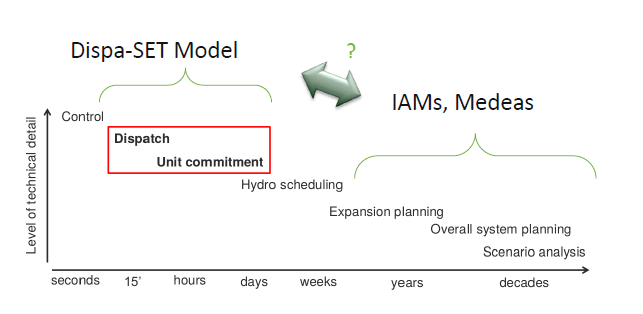
\includegraphics[width=0.8\textwidth]{resources/images/dispaset-medeas-timescale.png}
    \caption{An illustration of where Dispa-SET and MEDEAS operate on the timescale}
    \label{fig:dispaset-medeas-timescale}
\end{figure}

\subsubsection{Linking types}

There are several strategies that may be used in order to link two models together \cite{linkings-stuff}.

\begin{itemize}
    \item Soft linking: the models communicate between each other. This communication may be uni-directional or bi-directional. Both of the models are run iteratively, thus keeping their separate efficiencies in the same order of magnitude. However, the iteration lead to low overall speed, and convergence is not guaranteed.
    \item Hard linking: the models are combined into a single, unified mathematical formulation. This newly created model can then be solved all at once. This approach is burdened by higher computational costs and lower chance of feasibility.
\end{itemize}

These linking types are illustrated in Figure \ref{fig:linking-types}.

\begin{figure}[h]
    \centering
    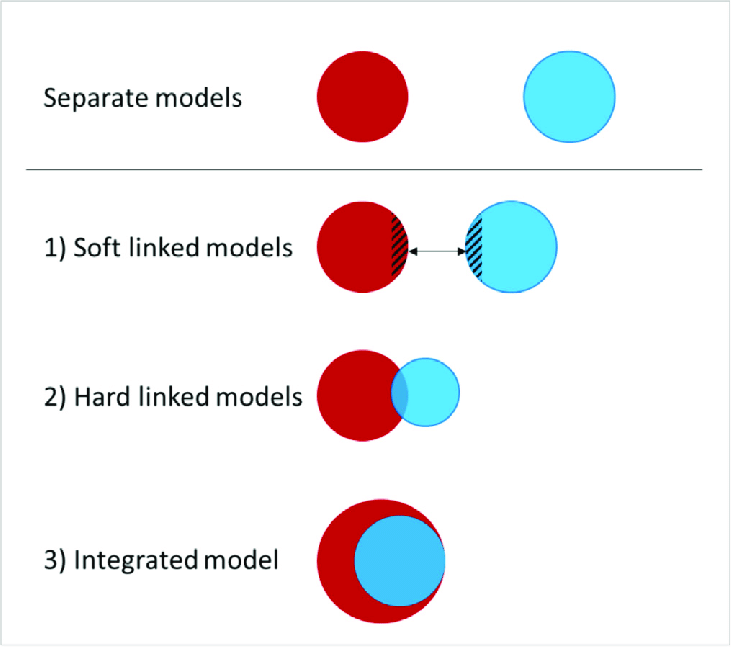
\includegraphics[width=0.4\textwidth]{resources/images/hybrid_model_variants.png}
    \caption{Illustration of the different linking methods \cite{hybrid_models}.}
    \label{fig:linking-types}
\end{figure}

One may also add model integration, consisting in completely embedding a model into the other. But this is not tractable in this setting, and would also requires compatible model formulations, as explained below.

In this case, hard linking is not possible owing to the different formulations of Dispa-SET (linear programming), and MEDEAS (system dynamics).

We also dismiss the soft linking strategy because of its slowness, and absence of convergence guarantee.

\subsubsection{Surrogate models}

Considering the effects of VRES in long-term integrated assessment models is a challenge since they don't have a sufficient time resolution to capture the rapid variations within the system.

The linking technique explored in this work is the surrogate model. In this case, an approximation of the Dispa-SET dispatch model is integrated into the MEDEAS IAM. 

The idea behind surrogate models is simple. First, a fast, convenient approximation of the model is made, then it its completely integrated in the other model. For this purpose, the relevant outputs of the Dispa-SET model is approximated from relevant inputs regarding MEDEAS, then the approximator is inserted in the model.

Similar work has been done by Parrado-Hernando et al. in \cite{Hernando2022}, that aims at "capturing features of hourly-resolution energy models". The methodology used to acquire the data presents two downsides that are addressed in this work.

First, the inputs of the energy model are handled as discrete variable, and simulation have been run using all possible combination for these values. This can be seen in some of their figures, where the data points seem to follow some lines. While it does not invalidate the process, this creates a bias in the repartition of the data. Second, linear approximation are used to fit the data obtained. Admittedly, this is identified as a limitation of the work.

To palliate these, the input space is tackled as a continuous domain for the design of experiment, and other machine learning technique are considered as to candidates for the creation of the surrogate model.

The soft-linking approach has already been explored \cite{Brinkerink2022-softlink}, \cite{DEane2012-softlink}, and the hard-linking remains the hardest to investigate, notably due to incompatible formulations. Surrogate models are still unexplored and are of great interest for this use case.

As the combination of the two models uses an approximation, this appriximation being fast will not burden the computations of the IAM, hence keeping it efficient.

Surrogate models then provide a promising strategy for the implementation of this integration problem.

\subsection{This work}

\subsubsection{Objective}

This master's thesis is dedicated to the integration of the flexibility constraints, the Dispa-SET surrogate model, into the MEDEAS model, with reduced details on this aspect. This includes the creation of a proper dataset, the definition, training and integration of the surrogate model into MEDEAS.
 
It extends previous work as such an approach, as discussed above, has not yet been implemented in this context.

\subsubsection{Contributions}

This work follows what was started by another student, Carla Vidal, that went until the surrogate model training, included. Given that improvements where implemented in Dispa-SET since then, the runs had to be re-done. However, there were no easy to use scripts to set up the simulation files etc., so that is has been chosen to write new ones.

Additionally, the present thesis also explores other machine learning algorithms, although the same choice of neural networks is made, this time based on better performance compared to the other options.

Another student, Jade Paris, was in responsible of the linking of the surrogate model, given as a functions of some inputs variables into the MEDEAS model, and its actual use and runs of MEDEAS with the surrogate model integrated.

This work constisted in:
\begin{itemize}
    \item The writing of scripts to run Dispa-SET on those experiments
    \item The choice, definition and implementation of an adequate machine learning model, and its training
    \item The integration the model in MEDEAS, by writing a C++ external function library for Vensim, or by inserting it into the PySD model of MEDEAS directly in python
    \item Runs and analysis of the improved MEDEAS model
\end{itemize}

The global workflow is depicted in Figure \ref{fig:thesis-workflow}.

\begin{figure}[h]
    \centering
    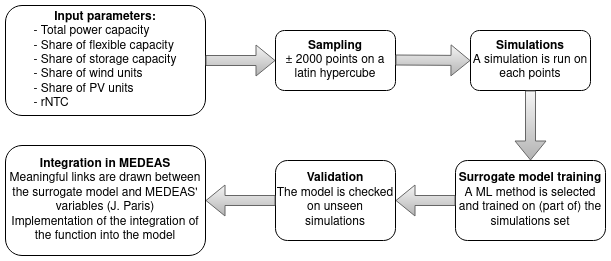
\includegraphics[width=0.7\textwidth]{resources/images/workflow.png}
    \caption{Worflow of the master thesis}
    \label{fig:thesis-workflow}
\end{figure}

All the produced work, and necessary data is available in the online github repository at the following address: \href{https://github.com/Rayerdyne/master-thesis}{https://github.com/Rayerdyne/master-thesis}.

\subsubsection{Outline}

This document is organized into seven main sections. The second section presents an in-depth description of the Dispa-SET model, along with the tools employed within its framework. Following this, the third section provides a detailed account of the MEDEAS model, outlining its underlying principles and the broader framework in which it operates.

To facilitate the successful integration of models, the fourth section outlines the process of data generation. This encompasses a complete overview of the methodologies employed to produce the necessary training data, the design of experiments and the execution of Dispa-SET runs.

Subsequently, the fifth section describes the surrogate model, offering a comprehensive description of its design. The section further expounds on the training and validation processes undertaken to ensure accurate alignment of the surrogate model with the main models' outcomes.

The sixth section then shifts the focus to the crucial process of integrating the surrogate model into MEDEAS. A step-by-step description is provided, elucidating how the surrogate model becomes an integral component of the broader MEDEAS framework, and how it interacts with the existing models.

In the seventh, the document offering a comprehensive summary of the resulting model and outcomes. This section also provides interpretations of the observed results.

Finally, the last section concludes, reflecting on the work and identifying any limitations and outlining future areas of research for further enhancements. 

% This document is structured as follows:

% \begin{enumerate}
%     \item \textbf{The Dispa-SET model}: description of the Dispa-SET model and tools
%     \item \textbf{The MEDEAS model}: description of the MEDEAS model and framework
%     \item \textbf{Data generation}: description of the complete process to generate the training data, that is, the design of experiments and the Dispa-SET runs
%     \item \textbf{The surrogate model}: definition of the surrogate model, training and validation
%     \item \textbf{Integration}: description of the process of integrating a model into MEDEAS
%     \item \textbf{Analysis}: the analysis of the runs of MEDEAS with the integrated surrogate model
%     \item \textbf{Conclusions}
% \end{enumerate}
